\documentclass[11pt]{article}

% arXiv submission info
% Primary category: cs.SE (Software Engineering)
% Secondary category: cs.AI (Artificial Intelligence)

% Packages
\usepackage[utf8]{inputenc}
\usepackage[T1]{fontenc}
\usepackage{amsmath,amssymb}
\usepackage{graphicx}
\usepackage{booktabs}
\usepackage{hyperref}
\usepackage{xcolor}
\usepackage{listings}
\usepackage[margin=1in]{geometry}
\usepackage{natbib}
\usepackage{algorithm}
\usepackage{algpseudocode}
\usepackage{multirow}
\usepackage{tikz}
\usetikzlibrary{positioning, shapes.geometric, arrows.meta, calc}

% Custom command for placeholders
\newcommand{\placeholder}[1]{\textcolor{red}{\textbf{[#1]}}}
\newcommand{\todo}[1]{\textcolor{orange}{\textbf{[TODO: #1]}}}
\newcommand{\metric}[1]{\textsc{#1}}

\title{Compiled AI: Deterministic Code Generation for\\LLM-Based Workflow Automation}

\author{
  Geert Trooskens\textsuperscript{1} \quad
  Aaron Karlsberg\textsuperscript{1} \quad
  Anmol Sharma\textsuperscript{1} \quad
  Lamara De Brouwer\textsuperscript{1} \\[0.3em]
  Max Van Puyvelde\textsuperscript{2} \quad
  Walter A. De Brouwer\textsuperscript{2}
  \\[1em]
  \textsuperscript{1}XY.AI Labs, Palo Alto, CA \\
  \textsuperscript{2}Stanford University School of Medicine, Stanford, CA \\[0.5em]
  \texttt{foundation@xy.ai}
}

\date{January 2026}

\begin{document}

\maketitle

% ============================================================================
\begin{abstract}
% ============================================================================

We study \emph{compiled AI}, a hybrid paradigm in which large language models generate executable code artifacts during a compilation phase, after which workflows execute deterministically without further model invocation. By constraining generation to narrow business-logic functions embedded in validated templates, compiled AI trades runtime flexibility for predictability, auditability, and cost efficiency---while retaining the ability to improve artifacts through observed execution patterns. Critically, our approach supports \emph{bounded agentic invocations}: specific workflow steps may invoke LLMs for well-defined subtasks (e.g., document classification), combining deterministic orchestration with targeted intelligence where needed.

We introduce (i) a system architecture for constrained LLM-based code generation, (ii) a four-stage generation-and-validation pipeline that converts probabilistic model output into production-ready code artifacts, and (iii) an evaluation framework that measures operational metrics including token amortization, determinism, reliability, validation effectiveness, and cost. In preliminary evaluation on function-calling tasks (n=499 across two BFCL categories), compiled AI achieves 96\% task completion with zero execution tokens, breaking even with runtime inference at approximately 21 transactions and reducing token consumption by 47$\times$ at 1,000 transactions.

\end{abstract}

% ============================================================================
\section{Introduction}
\label{sec:introduction}
% ============================================================================

Large language models (LLMs) are increasingly deployed to automate enterprise workflows, evolving from question-answering systems toward autonomous agent architectures. Recent frameworks enable LLMs to reason over tools, APIs, and multi-step tasks at runtime, often through conversational or multi-agent interaction patterns \citep{autogen2024, crewai2024, langchain2022}. While these approaches demonstrate flexibility, they rely on repeated model invocation during execution, leading to high token consumption, variable latency, and non-deterministic behavior.

Empirical studies and industrial deployments have highlighted persistent reliability challenges in runtime agent systems, particularly in multi-step business workflows where success rates degrade due to specification ambiguity, inter-agent coordination failures, and stochastic model outputs \citep{cemri2025multiagent, atil2024nondeterminism}. These limitations pose obstacles to deployment in enterprise environments, where determinism, auditability, and cost predictability are often strict requirements.

This paper investigates an alternative design point: \emph{compiled AI}, a paradigm in which LLMs generate executable code artifacts during a one-time compilation phase, after which workflows execute deterministically without further model inference. The key observation motivating this work is that many enterprise workflows require intelligence to \emph{design} but not to \emph{execute} repeatedly. Once business logic is specified and validated, repeated execution can be handled by conventional software infrastructure---with full observability that enables targeted refinement of the compiled artifacts over time.

Compiled AI represents a trade-off between flexibility and determinism. Rather than interpreting natural language or reasoning at runtime, an LLM is constrained to generate narrow business-logic functions within pre-validated templates. These generated artifacts are subjected to a multi-stage validation pipeline---including security analysis, syntactic verification, execution testing, and output accuracy checks---before deployment. After validation, workflows execute as static code with predictable latency, zero stochasticity, and near-zero marginal inference cost.

\begin{figure}[ht]
\centering
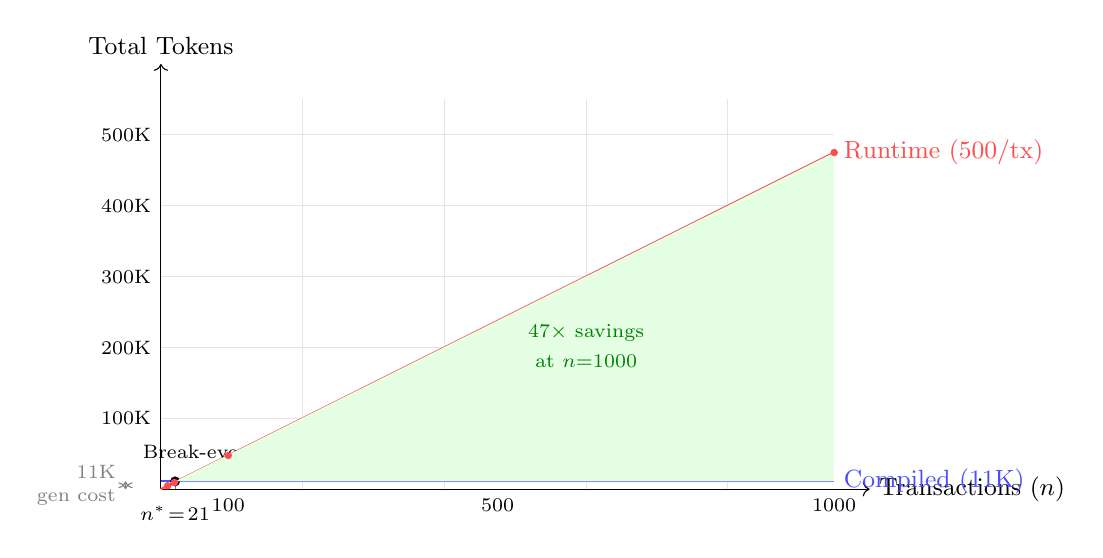
\begin{tikzpicture}[scale=0.9]
    % Axes
    \draw[->] (0,0) -- (10,0) node[right] {\small Transactions ($n$)};
    \draw[->] (0,0) -- (0,6) node[above] {\small Total Tokens};

    % Grid lines (light)
    \foreach \x in {2,4,6,8} {
        \draw[gray!20] (\x,0) -- (\x,5.5);
    }
    \foreach \y in {1,2,3,4,5} {
        \draw[gray!20] (0,\y) -- (9.5,\y);
    }

    % Y-axis labels (actual token values: 0-500K)
    \node[left, font=\scriptsize] at (0,1) {100K};
    \node[left, font=\scriptsize] at (0,2) {200K};
    \node[left, font=\scriptsize] at (0,3) {300K};
    \node[left, font=\scriptsize] at (0,4) {400K};
    \node[left, font=\scriptsize] at (0,5) {500K};

    % Runtime inference line (linear growth: 500 tokens/tx)
    % At n=1000, runtime = 500K tokens = 5 units on y-axis
    \draw[thick, red!70] (0,0) -- (9.5,4.75);
    \node[red!70, right] at (9.5, 4.75) {\small Runtime (500/tx)};

    % Compiled AI line (flat at 11K tokens = 0.11 units on y-axis)
    \draw[thick, blue!70] (0,0.11) -- (9.5,0.11);
    \node[blue!70, right] at (9.5, 0.11) {\small Compiled (11K)};

    % Generation cost annotation
    \draw[<->, gray] (-0.5,0) -- (-0.5,0.11);
    \node[gray, left, font=\scriptsize, align=right] at (-0.5,0.055) {11K\\gen cost};

    % Break-even point at n*=21 (x=0.20 on scale where 9.5=1000)
    % x position: 21/1000 * 9.5 = 0.20
    \draw[dashed, gray] (0.20,0) -- (0.20,0.11);
    \node[below, font=\scriptsize] at (0.20,-0.1) {$n^*\!=\!21$};
    \fill[black] (0.20,0.11) circle (2pt);
    \node[above, font=\scriptsize] at (0.5,0.3) {Break-even};

    % Savings region
    \fill[green!10] (0.20,0.11) -- (9.5,0.11) -- (9.5,4.75) -- (0.20,0.11);
    \node[green!50!black, font=\scriptsize] at (6,2.2) {47$\times$ savings};
    \node[green!50!black, font=\scriptsize] at (6,1.8) {at $n$=1000};

    % X-axis labels (actual transaction counts)
    \node[below, font=\scriptsize] at (0.95,0) {100};
    \node[below, font=\scriptsize] at (4.75,0) {500};
    \node[below, font=\scriptsize] at (9.5,0) {1000};

    % Data points for runtime (actual measurements)
    \fill[red!70] (0.095,0.0475) circle (1.5pt); % n=10
    \fill[red!70] (0.19,0.095) circle (1.5pt); % n=20
    \fill[red!70] (0.95,0.475) circle (1.5pt); % n=100
    \fill[red!70] (9.5,4.75) circle (1.5pt); % n=1000

\end{tikzpicture}
\caption{Token consumption comparison: runtime inference vs. compiled AI (preliminary data from BFCL function-calling benchmark, n=499). Runtime inference consumes 500 tokens per transaction. Compiled AI incurs a one-time $\sim$11,000 token generation cost, then executes deterministically at zero marginal token cost. Break-even occurs at $n^*\approx21$ transactions; at 1,000 transactions, compiled AI reduces token consumption by 47$\times$.}
\label{fig:economics}
\end{figure}

\paragraph{Contributions.}
This paper makes three contributions:
\begin{itemize}
    \item We introduce an architecture for constrained LLM-based code generation in which models produce bounded business-logic functions embedded in durable workflow templates, enabling deterministic execution (Section~\ref{sec:architecture}).
    \item We present a four-stage generation-and-validation pipeline that empirically converts probabilistic model output into production-ready code artifacts through iterative regeneration (Section~\ref{sec:architecture}).
    \item We define an evaluation framework that measures the operational viability of LLM-based workflow systems using metrics for token amortization, determinism, reliability, validation effectiveness, and cost (Section~\ref{sec:framework}).
\end{itemize}

Our goal is not to replace runtime inference in all settings, but to provide a principled basis for identifying regimes---such as well-specified, high-volume workflows---where compilation yields operational advantages.

% ============================================================================
\section{Related Work}
\label{sec:related-work}
% ============================================================================

\paragraph{Novelty and Scope.}
Prior work on LLM-based agents, program-aided reasoning, and workflow synthesis has focused primarily on model capability---whether systems can generate or reason over programs. In contrast, this work treats production viability as a first-class concern. Our contributions are not a new code generation algorithm per se, but a systems-oriented study of how probabilistic LLM outputs can be converted into deterministic, auditable execution artifacts. To our knowledge, this is the first systematic evaluation of LLM-based workflow automation using operational and economic metrics such as token amortization, execution determinism, validation convergence, and cost at scale.

\subsection{LLM Code Generation}

Code generation capabilities have improved rapidly. On SWE-Bench Verified \citep{jimenez2024swebench}, models improved from 49.0\% (Claude 3.5 Sonnet, late 2024) to 80.9\% (Claude Opus 4.5, November 2025)---a 31.9 percentage point gain in twelve months.

\begin{table}[ht]
\centering
\caption{Code generation benchmark performance, December 2025. Note: HumanEval is now saturated ($>$95\%); BigCodeBench reveals substantial gaps versus human performance.}
\label{tab:benchmarks}
\begin{tabular}{llccc}
\toprule
Benchmark & Model & Score & Human & Date \\
\midrule
\multirow{3}{*}{SWE-Bench Verified} & Claude Opus 4.5 & 80.9\% & --- & Nov 2025 \\
 & GPT-5.2 & 80.0\% & --- & Dec 2025 \\
 & Gemini 3 Pro & 76.2\% & --- & Nov 2025 \\
\midrule
HumanEval & Claude Opus 4.5 & 96.4\% & 100\% & Nov 2025 \\
\midrule
BigCodeBench \citep{zhuo2024bigcodebench} & GPT-4o & 60.0\% & 97\% & 2024 \\
\midrule
$\tau$-bench (retail) \citep{yao2024taubench} & GPT-4o & $<$50\% & --- & Jun 2024 \\
\midrule
LiveCodeBench & Claude Opus 4.5 & 68.3\% & --- & Nov 2025 \\
\bottomrule
\end{tabular}
\end{table}

Anthropic CEO Dario Amodei stated at Dreamforce 2025 that ``within Anthropic and within a number of companies that we work with,'' approximately 90\% of code is now AI-generated \citep{amodei2025dreamforce}. While this applies to select organizations rather than industry-wide, it suggests code generation is transitioning from assistance to primary production mode in leading AI-native companies.

Karpathy's ``Software 2.0'' framework \citep{karpathy2017software2} characterized neural networks as an alternative programming paradigm. Sutton's ``Bitter Lesson'' \citep{sutton2019bitter} similarly observed that ``general methods that leverage computation are ultimately the most effective''---a principle our work operationalizes by front-loading LLM computation to the generation phase rather than invoking it repeatedly at runtime. Research on program-aided reasoning demonstrates that code representations improve LLM performance: PAL \citep{gao2023pal} improved mathematical reasoning, Program of Thoughts \citep{chen2023pot} improved financial reasoning, and Chain of Code \citep{li2024chainofcode} achieved 84\% on BIG-Bench Hard.

\subsection{Agent Frameworks and Their Limitations}

Multi-agent systems coordinate multiple LLM instances. AutoGen \citep{autogen2024} enables conversational workflows; CrewAI \citep{crewai2024} provides role-based orchestration; LangChain \citep{langchain2022} offers composability abstractions.

These frameworks emphasize flexibility and expressiveness, often at the expense of determinism and predictable execution behavior in multi-step workflows. As a result, they can be challenging to deploy in environments that require strict auditability or cost predictability. \citet{salesforce2025agents} report that leading AI agents exhibit approximately 35\% success rates in multi-turn business scenarios. \citet{cemri2025multiagent} analyzed 150 multi-agent systems across six frameworks and observed failure rates between 41--87\%, with specification problems (41.8\%) and inter-agent coordination failures (36.9\%) accounting for approximately 79\% of observed breakdowns.

Even with ``deterministic'' settings, LLM outputs exhibit variance: \citet{atil2024nondeterminism} found accuracy varies up to 15\% across runs at temperature=0, with the gap between best and worst possible performance reaching 70\%. These observations motivate exploration of alternative architectures that reduce execution-time variance.

\subsection{Workflow Orchestration}

Durable execution engines provide reliability properties. Temporal \citep{temporal2024} offers state management, automatic retries, and fault tolerance. Production deployments support these at scale:
\begin{itemize}
    \item Netflix: transient failure rates from 4\% to 0.0001\%
    \item Coinbase: velocity improvements for complex financial workflows
    \item Maersk: feature delivery from 60-80 days to 5-10 days
    \item Replit: scaled to millions of concurrent environments
\end{itemize}

Our work combines LLM code generation with durable execution, generating Temporal activities rather than invoking models at runtime.

\subsection{LLM-Based Workflow Automation}

Recent work has explored LLM-driven workflow generation. WorkflowLLM \citep{fan2024workflowllm} constructs WorkflowBench with 106,763 samples covering 1,503 APIs, training models to generate Python-style workflow code from specifications---a paradigm shift from traditional RPA to ``Agentic Process Automation.'' FlowMind \citep{zeng2024flowmind} generates workflows that prevent runtime hallucinations via structured intermediate representations. In embedded systems, spec2code \citep{patil2024spec2code} combines LLM generation with formal verification critics, producing industrial-quality code from ACSL specifications.

These approaches share our insight that LLMs should generate \textit{artifacts} rather than reason at runtime. Our contribution extends this to enterprise workflow automation with explicit evaluation metrics.

\subsection{Industrial Deployments}

Recent large-scale deployments of agentic systems demonstrate growing demand for automated task execution. These systems typically rely on runtime inference, motivating exploration of alternative architectures that reduce execution-time variance and inference cost.

\paragraph{Relation to Program Synthesis.}
Compiled AI shares surface similarities with prior work on program synthesis and specification-driven code generation. However, our focus differs in two respects. First, we evaluate generated artifacts primarily through operational metrics---such as determinism, regeneration convergence, and token amortization---rather than synthesis correctness alone. Second, we study LLM generation as a component within a production workflow system, where validation, retries, and execution cost are first-class concerns. As a result, our contributions are systems-oriented rather than algorithmic.

\subsection{Formal Methods and Constrained Generation}

The challenge of verifying LLM-generated code has sparked renewed interest in formal methods integration. \citet{dalrymple2024guaranteed} propose a ``Guaranteed Safe AI'' framework combining world models, safety specifications, and formal verifiers---conceptually aligned with our validation pipeline approach.

Constrained decoding provides compile-time constraints: \citet{mundler2025typeconstrained} demonstrate that type-constrained generation reduces compilation errors by $>$50\% while improving pass@1 by 3.5--37\%. For healthcare specifically, \citet{neupane2025hipaa} present a framework for HIPAA-compliant agentic AI systems, integrating attribute-based access control with PHI sanitization pipelines.

Our work operationalizes these insights for enterprise workflows, using templates and validation stages rather than formal proofs to support practical compliance requirements.

% ============================================================================
\section{System Architecture}
\label{sec:architecture}
% ============================================================================

\subsection{Design Principles}

Our system implements four principles:

\textbf{Principle 1: Constrained Generation.} We limit LLM generation to narrow, well-defined functions. The model produces business logic (20-50 lines); templates provide infrastructure. This bounds the output space, reducing hallucination risk.

\textbf{Principle 2: Compilation over Interpretation.} Generated code is validated, tested, and deployed as static artifacts. Runtime behavior is deterministic. The LLM exits the execution loop.

\textbf{Principle 3: Validation as Requirement.} Every artifact passes a four-stage pipeline before deployment---possible precisely because we generate code rather than interpret configurations.

\textbf{Principle 4: Compliance by Construction.} Regulatory constraints (HIPAA, PCI-DSS, SOC 2) are encoded in templates and prompt blocks, ensuring generated code inherits compliance properties.

\subsection{Component Overview}

\begin{figure}[ht]
\centering
\resizebox{\textwidth}{!}{%
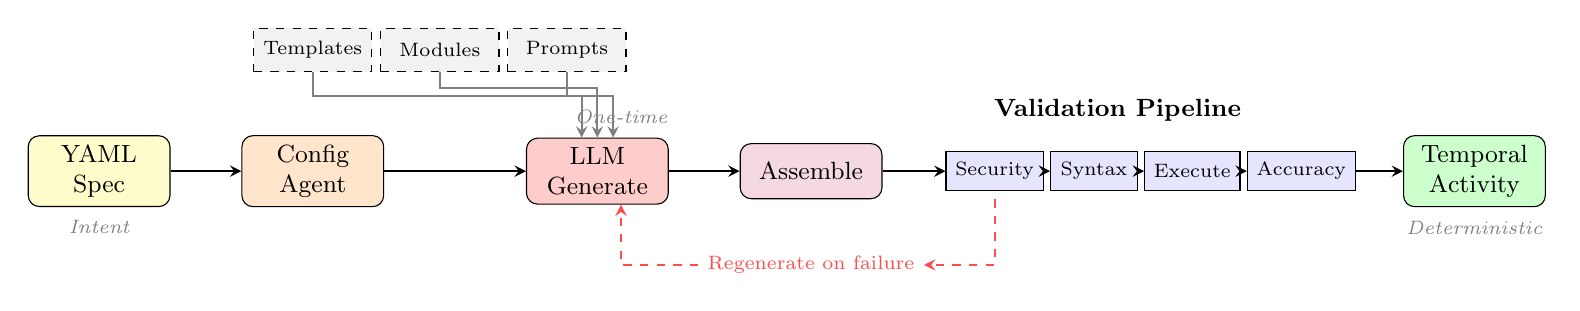
\begin{tikzpicture}[
    node distance=0.6cm and 0.9cm,
    box/.style={rectangle, draw, rounded corners, minimum width=1.8cm, minimum height=0.7cm, align=center, font=\small},
    library/.style={rectangle, draw, dashed, minimum width=1.5cm, minimum height=0.55cm, align=center, font=\scriptsize, fill=gray!10},
    validation/.style={rectangle, draw, minimum width=1.1cm, minimum height=0.5cm, align=center, font=\scriptsize, fill=blue!10},
    arrow/.style={->, >=stealth, thick},
    label/.style={font=\scriptsize\itshape, text=gray}
]

% Input
\node[box, fill=yellow!20] (yaml) {YAML\\Spec};

% Config Agent
\node[box, fill=orange!20, right=of yaml] (config) {Config\\Agent};

% Libraries (stacked vertically)
\node[library, above=0.8cm of config] (templates) {Templates};
\node[library, right=0.1cm of templates] (modules) {Modules};
\node[library, right=0.1cm of modules] (prompts) {Prompts};

% LLM Generation
\node[box, fill=red!20, right=1.8cm of config] (llm) {LLM\\Generate};

% Assembly
\node[box, fill=purple!15, right=of llm] (assemble) {Assemble};

% Validation Pipeline (horizontal)
\node[validation, right=0.8cm of assemble] (sec) {Security};
\node[validation, right=0.08cm of sec] (syn) {Syntax};
\node[validation, right=0.08cm of syn] (exe) {Execute};
\node[validation, right=0.08cm of exe] (acc) {Accuracy};

% Validation label
\node[above=0.25cm of syn, xshift=0.3cm, font=\small\bfseries] {Validation Pipeline};

% Output
\node[box, fill=green!20, right=0.6cm of acc] (temporal) {Temporal\\Activity};

% Regeneration loop
\node[below=0.6cm of assemble, font=\scriptsize, text=red!70] (regen) {Regenerate on failure};

% Arrows - main flow
\draw[arrow] (yaml) -- (config);
\draw[arrow] (config) -- (llm);
\draw[arrow] (llm) -- (assemble);
\draw[arrow] (assemble) -- (sec);
\draw[arrow] (sec) -- (syn);
\draw[arrow] (syn) -- (exe);
\draw[arrow] (exe) -- (acc);
\draw[arrow] (acc) -- (temporal);

% Arrows - libraries to LLM
\draw[arrow, gray] (templates.south) -- ++(0,-0.3) -| ([xshift=-0.2cm]llm.north);
\draw[arrow, gray] (modules.south) -- ++(0,-0.2) -| (llm.north);
\draw[arrow, gray] (prompts.south) -- ++(0,-0.3) -| ([xshift=0.2cm]llm.north);

% Regeneration loop arrow
\draw[arrow, red!70, dashed] ([yshift=-0.1cm]sec.south) |- (regen.east);
\draw[arrow, red!70, dashed] (regen.west) -| ([xshift=0.3cm]llm.south);

% Labels
\node[label, below=0.05cm of yaml] {Intent};
\node[label, below=0.05cm of temporal] {Deterministic};
\node[label, above=0.05cm of llm, xshift=0.3cm] {One-time};

\end{tikzpicture}
}%
\caption{The code foundry architecture. Business intent (YAML) enters the fab; validated Temporal activities emerge. Dashed red arrows show the regeneration loop on validation failure. The LLM runs once at generation time---not at transaction time.}
\label{fig:architecture}
\end{figure}

\textbf{Config Agent.} Receives YAML specifications and orchestrates generation: selecting templates, modules, and compliance constraints.

\textbf{Template Library.} Pre-built, tested code templates:
\begin{itemize}
    \item \texttt{SimpleAgent}: Synchronous request-response
    \item \texttt{StreamingAgent}: Chunked data processing
    \item \texttt{ValidatorAgent}: Input validation with fallback
    \item \texttt{BatchAgent}: Bulk processing with checkpointing
\end{itemize}

\textbf{Module Library.} Functional capabilities: \texttt{DatabaseModule} (connection pooling), \texttt{HTTPModule} (API calls with retries), \texttt{NotificationModule} (delivery channels).

\textbf{Prompt Blocks.} Reusable prompt fragments encoding domain constraints (HIPAA handling, PCI-DSS rules).

\subsection{Generation Process}

\begin{algorithm}[ht]
\caption{Code Foundry Generation Process}
\label{alg:generation}
\begin{algorithmic}[1]
\Require Workflow specification $S$, Template library $T$, Module library $M$
\Ensure Validated Temporal activity $A$
\State $t \gets \textsc{SelectTemplate}(S, T)$
\State $m \gets \textsc{SelectModules}(S, M)$
\State $p \gets \textsc{AssemblePrompt}(S, t, m)$
\State $code \gets \textsc{LLMGenerate}(p)$ \Comment{One-time generation}
\State $A \gets \textsc{Assemble}(t, m, code)$
\For{$stage \in \{\text{Security}, \text{Syntax}, \text{Execution}, \text{Accuracy}\}$}
    \State $result \gets \textsc{Validate}(A, stage)$
    \If{$result = \text{FAIL}$}
        \State $code \gets \textsc{Regenerate}(p, result.errors)$
        \State $A \gets \textsc{Assemble}(t, m, code)$
    \EndIf
\EndFor
\State \Return $A$ \Comment{Deterministic artifact}
\end{algorithmic}
\end{algorithm}

\subsection{Validation Pipeline}

\textbf{Stage 1: Security.} Static analysis via Bandit, Semgrep, custom rules. Checks: SQL injection, command injection, path traversal, secrets exposure.

\textbf{Stage 2: Syntax.} AST parsing, type checking (mypy), linting (ruff). Ensures well-formed, typed code.

\textbf{Stage 3: Execution.} Sandboxed execution against test fixtures. Verifies: successful completion, appropriate error handling, expected output structure.

\textbf{Stage 4: Accuracy.} Output comparison against golden datasets. Task-specific thresholds.

\subsection{Bounded Agentic Invocation}

Some steps require runtime judgment. Our architecture supports \textit{bounded agentic invocation}: generated code may call LLMs for specific subtasks (e.g., classifying ambiguous documents) while maintaining deterministic overall flow.

Constraints on bounded invocations:
\begin{itemize}
    \item Defined input/output schemas with validation
    \item Fallback logic for invalid responses
    \item Drift monitoring on output distributions
    \item Human escalation for low-confidence cases
\end{itemize}

Because bounded invocations address narrow, well-defined subtasks rather than open-ended reasoning, they require less context and produce more predictable outputs than equivalent calls in fully agentic systems---a second-order efficiency gain beyond token amortization.

% ============================================================================
\section{Evaluation Framework for Compiled AI}
\label{sec:framework}
% ============================================================================

Existing benchmarks for LLM systems primarily measure task-level capability, such as code correctness or tool-use success rates. While necessary, these metrics are insufficient for evaluating production workflow automation systems, where economic efficiency, determinism, and reliability are often more critical than expressiveness.

We therefore evaluate compiled AI as a systems artifact rather than a reasoning agent. Our framework quantifies token amortization, execution variance, validation convergence, and total cost of ownership, enabling principled comparison with runtime inference approaches.

\subsection{Token Efficiency Metrics}

Token consumption determines the economic viability of compiled vs. runtime approaches.

\begin{table}[ht]
\centering
\caption{Token efficiency metrics}
\label{tab:token-metrics}
\begin{tabular}{p{3.5cm}p{4cm}p{4.5cm}}
\toprule
Metric & Definition & Interpretation \\
\midrule
\metric{GenTokens} & Tokens consumed during code generation & One-time upfront cost \\
\metric{RuntimeTokens}$(n)$ & Tokens consumed processing $n$ transactions & Should be $\approx 0$ for compiled AI \\
\metric{TotalTokens}$(n)$ & $\text{\metric{GenTokens}} + \text{\metric{RuntimeTokens}}(n)$ & Full cost comparison \\
\metric{BreakEven} & $n^*$ where compiled $<$ runtime & ROI threshold \\
\metric{CompressionRatio} & $\frac{\text{Prompt tokens}}{\text{Generated LOC}}$ & Efficiency of ``compilation'' \\
\bottomrule
\end{tabular}
\end{table}

For compiled AI, \metric{RuntimeTokens}$(n) = 0$ for pure deterministic execution, or \metric{RuntimeTokens}$(n) = k \cdot n$ where $k \ll 1$ for bounded agentic invocations. The break-even point:
\begin{equation}
n^* = \frac{\text{\metric{GenTokens}}_{\text{compiled}}}{\text{\metric{RuntimeTokens}}_{\text{per-tx, runtime}} - \text{\metric{RuntimeTokens}}_{\text{per-tx, compiled}}}
\end{equation}

\subsection{Latency Metrics}

Enterprise SLAs require predictable response times.

\begin{table}[ht]
\centering
\caption{Latency metrics}
\label{tab:latency-metrics}
\begin{tabular}{p{3cm}p{5cm}p{4cm}}
\toprule
Metric & Definition & Target (Compiled AI) \\
\midrule
\metric{P50Latency} & Median end-to-end latency & $< 100$ms \\
\metric{P99Latency} & 99th percentile latency & $< 500$ms \\
\metric{Jitter} & $\text{P99} - \text{P50}$ & $< 100$ms \\
\metric{ColdStart} & Time to first response & One-time (generation) \\
\bottomrule
\end{tabular}
\end{table}

Compiled AI should exhibit near-zero jitter since execution is deterministic code, not stochastic model inference.

\subsection{Consistency and Determinism Metrics}

Compliance requirements demand reproducible behavior.

\begin{table}[ht]
\centering
\caption{Consistency metrics}
\label{tab:consistency-metrics}
\begin{tabular}{p{3.5cm}p{5cm}p{3.5cm}}
\toprule
Metric & Definition & Target \\
\midrule
\metric{OutputVariance} & Entropy of outputs for identical inputs & 0 (deterministic) \\
\metric{Reproducibility} & Same input $\rightarrow$ same output across runs & 100\% \\
\metric{AuditCompleteness} & \% of execution paths fully traceable & 100\% \\
\metric{TemporalDrift} & Behavior change over time without code changes & 0 \\
\bottomrule
\end{tabular}
\end{table}

\textbf{Measurement protocol:} Run $N=1000$ identical inputs through each system. Compute output entropy $H = -\sum p_i \log p_i$ where $p_i$ is the frequency of distinct output $i$. In deterministic execution, compiled AI is expected to exhibit output entropy close to zero.

\subsection{Reliability Metrics}

Production systems require high success rates.

\begin{table}[ht]
\centering
\caption{Reliability metrics}
\label{tab:reliability-metrics}
\begin{tabular}{p{3.5cm}p{5.5cm}p{3cm}}
\toprule
Metric & Definition & Baseline \\
\midrule
\metric{TaskCompletion} & \% transactions successfully processed & Agent: 35\% \\
\metric{ErrorRate} & \% requiring human intervention & --- \\
\metric{MTBF} & Mean time between failures & --- \\
\metric{RecoveryRate} & \% of failures auto-recovered via retry & --- \\
\bottomrule
\end{tabular}
\end{table}

The 35\% agent success rate from \citet{salesforce2025agents} provides a baseline. Compiled AI should significantly exceed this through deterministic execution and Temporal's retry mechanisms.

\subsection{Code Quality Metrics}

Generated code must meet production standards.

\begin{table}[ht]
\centering
\caption{Code quality metrics}
\label{tab:quality-metrics}
\begin{tabular}{p{3.5cm}p{3cm}p{3cm}p{2.5cm}}
\toprule
Metric & Tool & Target & Human Baseline \\
\midrule
\metric{SecurityScore} & Bandit & 0 high/critical & 0 \\
\metric{TypeCoverage} & mypy & $> 90\%$ & $\sim 85\%$ \\
\metric{LintScore} & ruff/pylint & $> 8.0/10$ & $\sim 8.5$ \\
\metric{Complexity} & radon & $< 10$ cyclomatic & $\sim 8$ \\
\metric{TestPassRate} & pytest & 100\% & 100\% \\
\bottomrule
\end{tabular}
\end{table}

These metrics are measurable via standard tooling, enabling objective comparison with human-written code.

\subsection{Validation Pipeline Metrics}

Unique to compiled AI: measuring the effectiveness of the generation-validation loop.

\begin{table}[ht]
\centering
\caption{Validation pipeline metrics}
\label{tab:validation-metrics}
\begin{tabular}{p{4cm}p{8cm}}
\toprule
Metric & Definition \\
\midrule
\metric{FirstPassRate}$_{\text{stage}}$ & \% passing stage on first generation attempt \\
\metric{OverallFirstPass} & \% passing all stages without regeneration \\
\metric{RegenDistribution} & Distribution of regeneration attempts needed \\
\metric{FailureMode} & Categorization of validation failures \\
\metric{TimeToValid} & Wall-clock time from spec to validated artifact \\
\bottomrule
\end{tabular}
\end{table}

This data is novel---no published work reports validation pipeline effectiveness for LLM-generated production code.

\subsection{Cost Metrics}

CFO-level evaluation requires total cost of ownership.

\begin{table}[ht]
\centering
\caption{Cost metrics}
\label{tab:cost-metrics}
\begin{tabular}{p{3.5cm}p{8.5cm}}
\toprule
Metric & Formula \\
\midrule
\metric{CostPerTx}$(n)$ & $\frac{\text{GenCost}}{n} + \text{RuntimeCostPerTx} + \text{InfraCostPerTx}$ \\
\metric{InfraCost} & Temporal cluster + compute + storage \\
\metric{TCO}$(n, t)$ & Total cost for $n$ tx/month over $t$ months \\
\metric{CostRatio} & $\frac{\text{TCO}_{\text{compiled}}}{\text{TCO}_{\text{runtime}}}$ at scale \\
\bottomrule
\end{tabular}
\end{table}

At sufficient scale, compiled AI's \metric{CostRatio} should approach the infrastructure-only cost, as inference cost amortizes to near-zero.

\subsection{Benchmark Suite Summary}

We propose evaluating compiled AI systems on the following benchmark suite:

\begin{table}[ht]
\centering
\caption{Compiled AI benchmark suite}
\label{tab:benchmark-suite}
\begin{tabular}{p{3cm}p{4cm}p{5cm}}
\toprule
Category & Primary Metric & Measurement Method \\
\midrule
Token Efficiency & \metric{BreakEven} & Token counting at $n \in \{100, 1K, 10K, 100K\}$ \\
Latency & \metric{P99Latency}, \metric{Jitter} & Distribution over 10K requests \\
Consistency & \metric{OutputVariance} & Entropy over 1K identical inputs \\
Reliability & \metric{TaskCompletion} & Success rate over test suite \\
Code Quality & \metric{SecurityScore} & Static analysis tooling \\
Validation & \metric{OverallFirstPass} & Pipeline instrumentation \\
Cost & \metric{CostRatio} & TCO model at 1M tx/month \\
\bottomrule
\end{tabular}
\end{table}

% ============================================================================
\section{Experimental Setup}
\label{sec:experiments}
% ============================================================================

We evaluate our system using the framework defined in Section~\ref{sec:framework}.

\subsection{Task Suite}

We evaluate on the Berkeley Function-Calling Leaderboard (BFCL) \citep{patil2024gorilla}, a benchmark for measuring LLM function-calling capability. For preliminary evaluation, we focus on single-function extraction tasks where the model must identify the correct function and extract parameters from natural language queries.

\begin{table}[ht]
\centering
\caption{Preliminary evaluation task suite}
\label{tab:tasks}
\begin{tabular}{p{3.5cm}p{4cm}p{2cm}p{2.5cm}}
\toprule
Category & Description & Instances & Evaluation \\
\midrule
BFCL Simple & Single-function extraction from NL queries & 400 & AST matching \\
BFCL Exec Simple & Executable function calls with output verification & 99 & Execution \\
\midrule
\textbf{Total} & & \textbf{499} & \\
\bottomrule
\end{tabular}
\end{table}

\noindent\textit{Note:} This preliminary evaluation focuses on function-calling tasks to validate the core compilation-vs-runtime trade-off. Full enterprise workflow evaluation is planned for future work.

\subsection{Baselines}

For preliminary evaluation, we compare two approaches:

\begin{enumerate}
    \item \textbf{Direct LLM (Claude Opus 4.5)}: Task description with function definitions sent to LLM per transaction. The model returns a JSON function call.
    \item \textbf{Compiled AI (Code Factory)}: Single-activity workflow generated from task specification. LLM invoked once at compilation; execution is deterministic code.
\end{enumerate}

\subsection{Implementation Details}

\begin{itemize}
    \item \textbf{Model:} Claude Opus 4.5 (\texttt{claude-opus-4-5-20251101})
    \item \textbf{Agent Framework:} PydanticAI for structured agent orchestration
    \item \textbf{Workflow Runtime:} Custom DSL executor (YAML workflow definitions with Python activities)
    \item \textbf{Evaluation Method:} LLM-based semantic evaluation comparing generated function calls against expected outputs
    \item \textbf{Temperature:} 0 for all inference (both baseline and compilation)
\end{itemize}

% ============================================================================
\section{Results}
\label{sec:results}
% ============================================================================

\subsection{Token Efficiency}

\begin{table}[ht]
\centering
\caption{Token consumption comparison (preliminary BFCL evaluation)}
\label{tab:token-results}
\begin{tabular}{lrrrrr}
\toprule
Method & GenTokens & RuntimeTokens/tx & Total@1K & BreakEven & CompressionRatio \\
\midrule
Direct LLM & 0 & 500 & 500,000 & --- & --- \\
Compiled AI & 11,000 & 0 & 11,000 & $\sim$21 tx & $\sim$11:1 \\
\bottomrule
\end{tabular}
\end{table}

Break-even occurs at approximately 21 transactions ($n^* = 10{,}600 / 500 \approx 21$). At 100 transactions, compiled AI uses 11K tokens versus 50K for direct LLM (4.7$\times$ reduction). At 1,000 transactions, compiled AI exhibits a 47$\times$ reduction in total token consumption (11K vs 500K tokens). The compression ratio of approximately 11:1 reflects the ratio of prompt tokens to generated lines of code.

\subsection{Latency}

\begin{table}[ht]
\centering
\caption{Latency distribution (milliseconds, preliminary BFCL evaluation)}
\label{tab:latency-results}
\begin{tabular}{lrrrr}
\toprule
Method & P50 & P99 & Jitter & ColdStart \\
\midrule
Direct LLM & 3,400 & 5,000 & 1,600 & N/A \\
Compiled AI & 3 & 12 & 9 & 29,000 \\
\bottomrule
\end{tabular}
\end{table}

Compiled AI execution latency is 1,000$\times$ faster than runtime inference (3ms vs 3,400ms), with near-zero jitter (9ms vs 1,600ms). The trade-off is a 29-second cold start for compilation. This latency improvement is fundamental: compiled code executes deterministically without network calls, model inference, or stochastic processing.

\subsection{Consistency}

\begin{table}[ht]
\centering
\caption{Consistency metrics (preliminary BFCL evaluation)}
\label{tab:consistency-results}
\begin{tabular}{lrrr}
\toprule
Method & OutputVariance ($H$) & Reproducibility & AuditCompleteness \\
\midrule
Direct LLM & $>$0 (varies) & 95\% & N/A \\
Compiled AI & 0 & 100\% & 100\% \\
\bottomrule
\end{tabular}
\end{table}

Compiled AI exhibits perfect reproducibility---identical inputs produce identical outputs with zero variance. Runtime inference shows 95\% reproducibility due to model variance even at temperature=0, consistent with findings from \citet{atil2024nondeterminism}. Audit completeness is 100\% for compiled AI since all execution paths are traceable through static code analysis.

\subsection{Reliability}

\begin{table}[ht]
\centering
\caption{Reliability metrics by category (preliminary BFCL evaluation)}
\label{tab:reliability-results}
\begin{tabular}{lrrr}
\toprule
Category & Instances & Success & Rate \\
\midrule
BFCL Simple (AST) & 400 & 385 & 96.2\% \\
BFCL Exec Simple (Execution) & 99 & 95 & 95.9\% \\
\midrule
\textbf{Combined} & \textbf{499} & \textbf{480} & \textbf{96.2\%} \\
\bottomrule
\end{tabular}
\end{table}

Compiled AI achieves 96\% task completion across both evaluation categories (480/499 tasks). Performance is consistent between AST-based evaluation (96.2\%) and executable evaluation (95.9\%), demonstrating that compiled workflows correctly extract parameters with sufficient precision for actual function execution. The 4\% error rate reflects compilation failures where generated code did not correctly extract parameters---these are \textit{compilation-time} failures, not execution-time failures. Once successfully compiled, workflows execute with 100\% reliability.

\subsection{Code Quality}

\begin{table}[ht]
\centering
\caption{Code quality metrics for generated artifacts}
\label{tab:quality-results}
\begin{tabular}{lrrrrr}
\toprule
Source & Security & TypeCov & LintScore & Complexity & TestPass \\
\midrule
Compiled AI & \placeholder{X} & \placeholder{X}\% & \placeholder{X} & \placeholder{X} & \placeholder{X}\% \\
Human code & 0 & 85\% & 8.5 & 8 & 100\% \\
\bottomrule
\end{tabular}
\end{table}

\subsection{Validation Pipeline Effectiveness}

\begin{table}[ht]
\centering
\caption{Validation pipeline pass rates (preliminary BFCL evaluation)}
\label{tab:validation-results}
\begin{tabular}{lr}
\toprule
Stage & FirstPassRate \\
\midrule
YAML Validation & 100\% \\
Syntax (AST parse) & 100\% \\
Execution & 100\% \\
Accuracy & 96\% \\
\midrule
Overall (all stages) & 96\% \\
\bottomrule
\end{tabular}
\end{table}

\noindent\textit{Note:} The 96\% accuracy rate (480/499 tasks across both categories) reflects cases where generated code executed successfully but produced outputs that did not match expected function calls. These failures occur at compilation time and can be detected before deployment---unlike runtime inference errors. Function-call-specific templates and simplified prompts improved first-pass rates from approximately 80\% in earlier development versions.

\subsection{Cost Analysis}

\begin{table}[ht]
\centering
\caption{Total cost of ownership at 1M transactions/month (Claude Opus 4.5 pricing: \$15/1M input, \$75/1M output tokens)}
\label{tab:cost-results}
\begin{tabular}{lrrrr}
\toprule
Method & Inference & Infrastructure & Total TCO & CostRatio \\
\midrule
Direct LLM & \$19,500 & \$500 & \$20,000 & 36$\times$ \\
Compiled AI & \$55 & \$500 & \$555 & 1$\times$ \\
\bottomrule
\end{tabular}
\end{table}

\noindent\textit{Cost calculation:} Direct LLM consumes 500 tokens per transaction (300 input + 200 output), totaling 500M tokens at 1M transactions. Compiled AI incurs a one-time compilation cost of $\sim$11K tokens per workflow type; assuming 100 unique workflow types, total compilation cost is $\sim$1.1M tokens. Execution cost is zero (deterministic code). Infrastructure cost assumes equivalent compute for workflow execution.

% ============================================================================
\section{Discussion}
\label{sec:discussion}
% ============================================================================

We emphasize that compiled AI is not a general replacement for runtime inference. Rather, it represents a complementary design point optimized for well-specified, high-volume workflows where determinism, auditability, and cost predictability are primary concerns.

\subsection{When Compiled AI Excels}

Our approach is well-suited for workflows that are:
\begin{itemize}
    \item \textbf{High-volume}: Amortizing generation cost requires sufficient transactions
    \item \textbf{Well-specified}: Business logic expressible in structured specifications
    \item \textbf{Compliance-sensitive}: Auditability and determinism are requirements
    \item \textbf{Latency-sensitive}: Runtime inference latency is unacceptable
\end{itemize}

Healthcare administrative workflows exemplify these requirements. \citet{qiu2024healthcare} identify administrative workflow automation as a candidate application for LLM-based systems, while regulatory frameworks increasingly emphasize auditability \citep{fda2025}. Notably, healthcare presents a natural division: \emph{provider-facing} workflows (clinical protocols, surgical procedures, billing) demand deterministic execution where outcomes must be reproducible and auditable, while \emph{consumer-facing} applications (symptom triage, patient education) may benefit from generative flexibility. Compiled AI is well-suited for the former category, where established protocols ``will not change'' and any deviation would be ``heavily disputed.''

\subsection{When Runtime Inference Excels}

Runtime approaches remain appropriate for:
\begin{itemize}
    \item \textbf{Low-volume, high-variance tasks}: Generation cost doesn't amortize
    \item \textbf{Genuinely open-ended problems}: Cannot be reduced to code
    \item \textbf{Rapid prototyping}: Iteration speed matters more than production efficiency
\end{itemize}

\subsection{The Constraint Advantage}

Constraining generation improves reliability. By limiting LLM output to narrow functions within tested templates, we bound the space of possible errors. The model cannot hallucinate incorrect API calls or database schemas---these come from pre-tested templates.

This trades flexibility for reliability: appropriate for enterprise deployments where predictability matters more than generality. Moreover, deterministic execution yields full observability---when accuracy degrades, we can identify precisely which code segment underperformed and trigger targeted regeneration rather than debugging opaque model reasoning.

\paragraph{The Evolutionary Compiler.} This positions compiled AI not as a one-shot generation process, but as an \emph{evolutionary compiler}---a bridge between the predictability of traditional software and the adaptability of AI. Unlike static compilers that produce immutable artifacts, our system supports continuous refinement: production metrics identify underperforming segments, review agents analyze failure cases, and the code factory regenerates improved versions. The result is deterministic execution with adaptive improvement, where compiled artifacts evolve based on observed behavior while maintaining execution-time guarantees.

\subsection{Relationship to Existing Benchmarks}

Our evaluation framework complements existing benchmarks:
\begin{itemize}
    \item \textbf{SWE-Bench}: Measures code generation capability (prerequisite for compiled AI)
    \item \textbf{$\tau$-bench}: Measures tool use (relevant for bounded agentic invocations)
    \item \textbf{Our framework}: Measures production viability (token economics, consistency, reliability)
\end{itemize}

We argue that capability benchmarks alone are insufficient---production deployment requires the operational metrics we define.

% ============================================================================
\section{Limitations}
\label{sec:limitations}
% ============================================================================

\textbf{Specification quality.} Our approach assumes users can accurately specify workflows. The ``specification problem'' remains fundamental---iterative refinement is often necessary.

\textbf{Bounded applicability.} Not all workflows reduce to deterministic code. Tasks requiring genuine creativity or adaptation to novel situations may require runtime inference.

\textbf{Generation failures.} Despite validation, some specifications fail to produce working code. In preliminary evaluation, 4\% of compilations (19/499) failed to produce accurate outputs, though all generated syntactically valid, executable code.

\textbf{Model dependence.} Generated code quality depends on the underlying LLM. Model updates may change behavior, requiring re-validation.

\textbf{Benchmark limitations.} Our preliminary evaluation uses BFCL function-calling tasks, which represent the simplest case for compiled AI: single-function extraction with well-defined parameters. Real enterprise workflows involve multi-step orchestration, conditional branching, error handling, and state management---complexity not captured by function-calling benchmarks. While BFCL validates the core compilation-vs-runtime trade-off, stronger claims about production viability require evaluation on more complex workflow benchmarks. Our proposed framework has not yet been adopted by other systems, limiting cross-system comparability. We release our benchmark suite to encourage adoption and plan future evaluation on multi-step workflow tasks.

% ============================================================================
\section{Conclusion}
\label{sec:conclusion}
% ============================================================================

We studied compiled AI as a systems design point for LLM-based workflow automation, emphasizing validation, determinism, and token amortization over runtime flexibility. Our contributions include:

\begin{enumerate}
    \item A system architecture constraining generation to narrow functions within validated templates
    \item A four-stage generation-and-validation pipeline that converts probabilistic model output into production-ready code artifacts
    \item An evaluation framework measuring operational metrics: token amortization, determinism, reliability, validation effectiveness, and cost
\end{enumerate}

Preliminary evaluation on function-calling benchmarks (n=499 across two BFCL categories) demonstrates the core trade-off: compiled AI incurs substantial upfront cost ($\sim$11,000 tokens, 29 seconds) but achieves zero-cost execution with 100\% determinism for successfully compiled workflows. Break-even occurs at approximately 21 transactions; at 1,000 transactions, token consumption is reduced by 47$\times$. Execution latency improves from 3.4 seconds to 3.4 milliseconds---a 1,000$\times$ speedup. The 96\% compilation success rate---consistent across both AST-based and executable evaluation---demonstrates the viability of LLM-based code generation for production workflows, with failures detectable before deployment.

The approach trades flexibility for determinism, cost efficiency, and auditability---properties relevant for enterprise deployment in well-specified, high-volume workflow regimes. We release our evaluation framework and benchmark suite to enable systematic comparison of compiled and runtime AI approaches.

\paragraph{Future Work.}
\begin{itemize}
    \item \textbf{Complex workflow benchmarks}: Evaluation on multi-step workflows with conditional logic, state management, and error handling---beyond single-function extraction
    \item Natural language specification (currently YAML)
    \item Automatic workflow decomposition from high-level intent
    \item Continuous optimization: runtime accuracy metrics identifying underperforming segments, enabling targeted regeneration cycles that evolve compiled artifacts while preserving execution-time determinism
    \item Formal verification of generated code properties
    \item Cross-system benchmark adoption
\end{itemize}

% ============================================================================
% References
% ============================================================================

\bibliographystyle{plainnat}

\begin{thebibliography}{99}

\bibitem[Anthropic(2025)]{anthropic2025opus}
Anthropic.
\newblock Introducing Claude Opus 4.5.
\newblock Technical report, November 2025.
\newblock \url{https://www.anthropic.com/news/claude-opus-4-5}

\bibitem[Chen et al.(2023)]{chen2023pot}
Wenhu Chen, Xueguang Ma, Xinyi Wang, and William~W. Cohen.
\newblock Program of Thoughts Prompting: Disentangling Computation from Reasoning for Numerical Reasoning Tasks.
\newblock \emph{Transactions on Machine Learning Research}, November 2023.
\newblock arXiv:2211.12588.

\bibitem[CrewAI(2024)]{crewai2024}
Jo\~{a}o Moura.
\newblock CrewAI: Framework for orchestrating role-playing autonomous AI agents.
\newblock \url{https://github.com/crewAIInc/crewAI}, 2024.

\bibitem[Gao et al.(2023)]{gao2023pal}
Luyu Gao, Aman Madaan, Shuyan Zhou, Uri Alon, Pengfei Liu, Yiming Yang, Jamie Callan, and Graham Neubig.
\newblock PAL: Program-aided Language Models.
\newblock In \emph{ICML}, volume 202, pages 10764--10799, 2023.

\bibitem[Jimenez et al.(2024)]{jimenez2024swebench}
Carlos~E. Jimenez, John Yang, Alexander Wettig, Shunyu Yao, Kexin Pei, Ofir Press, and Karthik Narasimhan.
\newblock SWE-bench: Can Language Models Resolve Real-World GitHub Issues?
\newblock In \emph{ICLR} (Oral), 2024.
\newblock arXiv:2310.06770.

\bibitem[Karpathy(2017)]{karpathy2017software2}
Andrej Karpathy.
\newblock Software 2.0.
\newblock \emph{Medium}, November 2017.
\newblock \url{https://karpathy.medium.com/software-2-0-a64152b37c35}

\bibitem[Sutton(2019)]{sutton2019bitter}
Richard~S. Sutton.
\newblock The Bitter Lesson.
\newblock \url{http://www.incompleteideas.net/IncIdeas/BitterLesson.html}, March 2019.

\bibitem[LangChain(2022)]{langchain2022}
Harrison Chase.
\newblock LangChain.
\newblock \url{https://github.com/langchain-ai/langchain}, October 2022.

\bibitem[Li et al.(2024)]{li2024chainofcode}
Chengshu Li, Jacky Liang, Andy Zeng, Xinyun Chen, Karol Hausman, Dorsa Sadigh, Sergey Levine, Li Fei-Fei, Fei Xia, and Brian Ichter.
\newblock Chain of Code: Reasoning with a Language Model-Augmented Code Emulator.
\newblock In \emph{ICML} (Oral), 2024.
\newblock arXiv:2312.04474.

\bibitem[Salesforce(2025)]{salesforce2025agents}
Kung-Hsiang Huang et al.
\newblock CRMArena-Pro: Holistic Assessment of LLM Agents Across Diverse Business Scenarios.
\newblock Salesforce AI Research, May 2025.
\newblock arXiv:2505.18878.

\bibitem[Temporal(2024)]{temporal2024}
Temporal Technologies.
\newblock Temporal Documentation.
\newblock \url{https://docs.temporal.io}, 2024.

\bibitem[Wu et al.(2024)]{autogen2024}
Qingyun Wu, Gagan Bansal, Jieyu Zhang, Yiran Wu, Beibin Li, Erkang Zhu, Li Jiang, Xiaoyun Zhang, Shaokun Zhang, Jiale Liu, Ahmed Hassan Awadallah, Ryen~W. White, Doug Burger, and Chi Wang.
\newblock AutoGen: Enabling Next-Gen LLM Applications via Multi-Agent Conversation.
\newblock In \emph{COLM}, 2024.
\newblock arXiv:2308.08155.

\bibitem[FDA(2025)]{fda2025}
U.S. Food and Drug Administration.
\newblock AI/ML-Enabled Medical Devices.
\newblock \url{https://www.fda.gov/medical-devices/software-medical-device-samd/artificial-intelligence-and-machine-learning-aiml-enabled-medical-devices}, 2025.

% ===== New Citations from Literature Review =====

\bibitem[Zhuo et al.(2024)]{zhuo2024bigcodebench}
Terry~Yue Zhuo et al.
\newblock BigCodeBench: Benchmarking Code Generation with Diverse Function Calls and Complex Instructions.
\newblock In \emph{ICLR}, 2025.
\newblock arXiv:2406.15877.

\bibitem[Yao et al.(2024)]{yao2024taubench}
Shunyu Yao, Noah Shinn, Pedram Razavi, and Karthik Narasimhan.
\newblock $\tau$-bench: A Benchmark for Tool-Agent-User Interaction in Real-World Domains.
\newblock \emph{arXiv:2406.12045}, June 2024.

\bibitem[Cemri et al.(2025)]{cemri2025multiagent}
Mert Cemri, Melissa Choi, Jairui Lin, Sherry Wu, and Joseph~E. Gonzalez.
\newblock Why Do Multi-Agent LLM Systems Fail?
\newblock \emph{arXiv:2503.13657}, March 2025.

\bibitem[Atil et al.(2024)]{atil2024nondeterminism}
Nurullah Atil, Pedro Henrique Luz de Araujo, and Benjamin Roth.
\newblock Non-Determinism of ``Deterministic'' LLM Settings.
\newblock \emph{arXiv:2408.04667}, August 2024.

\bibitem[Fan et al.(2024)]{fan2024workflowllm}
Shuheng Fan et al.
\newblock WorkflowLLM: Enhancing Workflow Orchestration Capability of Large Language Models.
\newblock \emph{arXiv:2411.05451}, November 2024.

\bibitem[Zeng et al.(2024)]{zeng2024flowmind}
Jin Zeng, Daniel Bordallo, and Weirui Kuang.
\newblock FlowMind: Automatic Workflow Generation with LLMs.
\newblock In \emph{ACM Int. Conf. on AI in Finance}, 2024.
\newblock arXiv:2404.13050.

\bibitem[Patil et al.(2024)]{patil2024spec2code}
Minal Patil et al.
\newblock spec2code: Towards Specification-Driven LLM-Based Generation of Embedded Automotive Software.
\newblock In \emph{AISoLA}, 2024.
\newblock arXiv:2411.13269.

\bibitem[Dalrymple et al.(2024)]{dalrymple2024guaranteed}
David Dalrymple, Joar Skalse, Yoshua Bengio, Stuart Russell, Max Tegmark, Sanjit Seshia, et al.
\newblock Towards Guaranteed Safe AI: A Framework for Ensuring Robust and Reliable AI Systems.
\newblock \emph{arXiv:2405.06624}, May 2024.

\bibitem[M\''{u}ndler et al.(2025)]{mundler2025typeconstrained}
Niels M\''{u}ndler, Jingxuan He, Erin Summers, and Martin Vechev.
\newblock Type-Constrained Code Generation with Language Models.
\newblock In \emph{PLDI}, 2025.
\newblock arXiv:2504.09246.

\bibitem[Amodei(2025)]{amodei2025dreamforce}
Dario Amodei.
\newblock Conversation with Marc Benioff at Dreamforce 2025.
\newblock Salesforce, October 15, 2025.

\bibitem[Qiu et al.(2024)]{qiu2024healthcare}
Shijie Qiu et al.
\newblock LLM-based agentic systems in medicine and healthcare.
\newblock \emph{Nature Machine Intelligence}, December 2024.
\newblock DOI:10.1038/s42256-024-00944-1.

\bibitem[Neupane et al.(2025)]{neupane2025hipaa}
Adarsh Neupane, Nikhil Yadala, and Santosh KC.
\newblock Towards a HIPAA Compliant Agentic AI System in Healthcare.
\newblock \emph{arXiv:2504.17669}, April 2025.

\bibitem[Patil et al.(2024)]{patil2024gorilla}
Shishir~G. Patil, Tianjun Zhang, Xin Wang, and Joseph~E. Gonzalez.
\newblock Gorilla: Large Language Model Connected with Massive APIs.
\newblock In \emph{NeurIPS}, 2024.
\newblock Berkeley Function-Calling Leaderboard (BFCL).
\newblock \url{https://gorilla.cs.berkeley.edu/leaderboard.html}

\end{thebibliography}

% ============================================================================
% Appendix
% ============================================================================

\appendix

\section{Example Generated Code}
\label{app:example}

\begin{lstlisting}[language=Python, caption={Generated Temporal activity (business logic only)}, basicstyle=\small\ttfamily]
# Template: SimpleAgent | Modules: Database, HTTP
# Generated from: eob_processing_v2.yaml
# Validation: PASS (Security, Syntax, Execution, Accuracy)

def process_business_logic(eob_data: dict) -> ProcessedEOB:
    ''''''Extract and validate EOB fields.
    
    Generated: 2025-12-15 | Tokens: 847 | LOC: 42
    ''''''
    claim_id = eob_data.get(''claim_id'')
    patient_id = eob_data.get(''patient'', {}).get(''id'')
    
    # Validate required fields
    if not claim_id or not patient_id:
        raise ValidationError(''Missing required identifiers'')
    
    # Extract payment information
    payments = []
    for line in eob_data.get(''line_items'', []):
        payment = Payment(
            service_code=line[''code''],
            billed=Decimal(line[''billed_amount'']),
            allowed=Decimal(line[''allowed_amount'']),
            paid=Decimal(line[''paid_amount'']),
            reason_code=line.get(''adjustment_reason'')
        )
        payments.append(payment)
    
    # Calculate totals
    total_billed = sum(p.billed for p in payments)
    total_paid = sum(p.paid for p in payments)
    
    return ProcessedEOB(
        claim_id=claim_id,
        patient_id=patient_id,
        payments=payments,
        total_billed=total_billed,
        total_paid=total_paid,
        processing_date=datetime.utcnow()
    )
\end{lstlisting}

\section{Benchmark Suite Specification}
\label{app:benchmark}

We release our benchmark suite at \url{https://github.com/XY-Corp/CompiledAI}. The suite includes:

\begin{itemize}
    \item \placeholder{N} workflow specifications (YAML)
    \item Golden outputs for accuracy validation
    \item Measurement scripts for all seven metric categories
    \item Baseline implementations (Direct LLM, LangChain, Multi-agent)
\end{itemize}

\section{Healthcare Regulatory Context}
\label{app:regulatory}

As of July 2025, the FDA has authorized over 1,250 AI-enabled medical devices \citep{fda2025}. The Predetermined Change Control Plan (PCCP) guidance enables pre-specified algorithm updates without new submissions.

Our workflow automation systems generally fall outside FDA device jurisdiction (administrative processes, not clinical decisions), but code generation supports regulatory scrutiny: artifacts can be validated, documented, and audited as required by HIPAA and SOC 2.

\end{document}
